\section{The JLAB Facility at 12 GeV}
\label{jlab}

\noindent The Jefferson Lab continuous wave electron accelerator facility (CEBAF) is designed from
two linear accelerators based
on superconducting radio frequency (RF) technology. Spin polarized electrons are generated in the gun
and pre-accelerated and accelerated in the north linac. They are then bent in a 180 degrees arc and injected
into the south linac.

\begin{figure}[h]
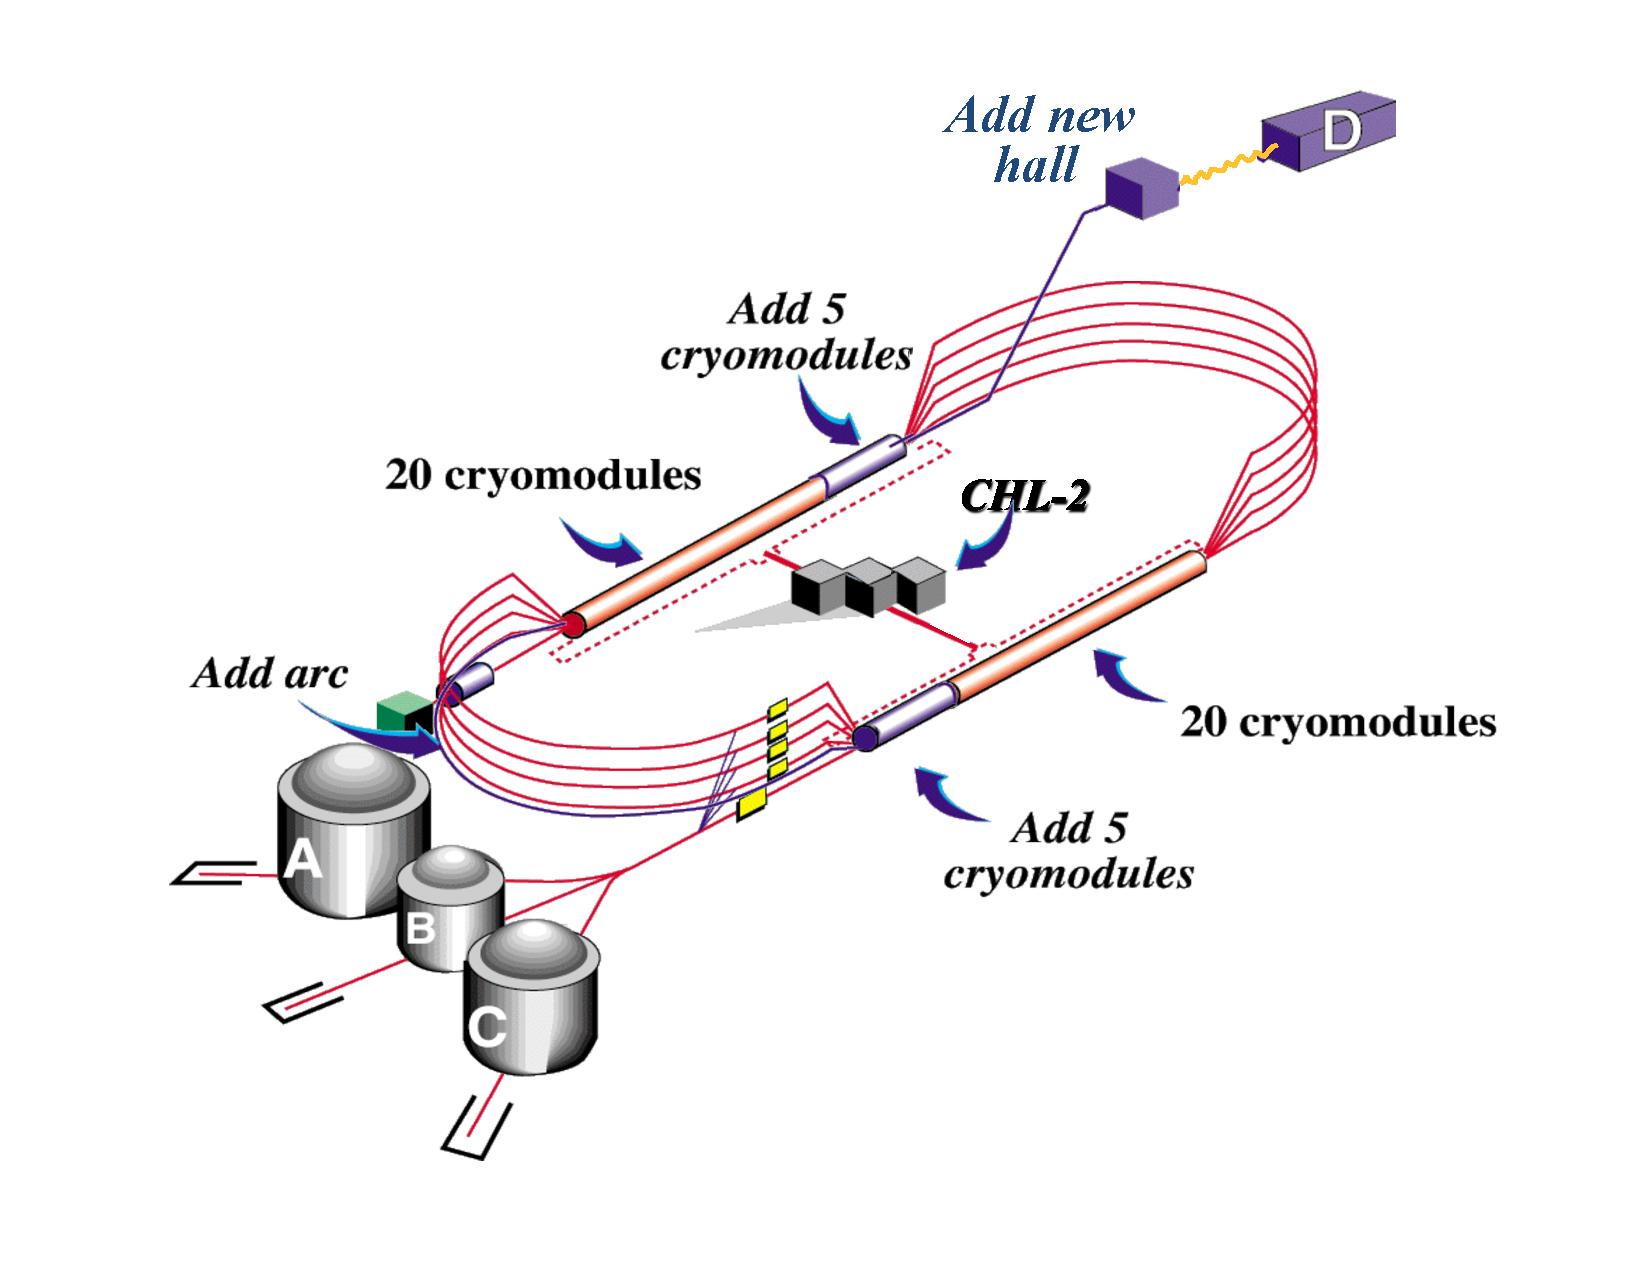
\includegraphics[width=1.0\columnwidth]{cebaf.pdf}
\caption{The CEBAF continuos electron beam accelerator after the doubling of the beam energy to 12 GeV and
adding Hall D as a new experimental end station for photon physics experiments. }
\end{figure}
This is repeated four and a half more times to reach the final energy for Hall D and up to four more passes
for desired delivery energies to Halls A, B and C. In the recirculating arcs, electrons are transported in 5
independent out-of-phase tracks of different energies. For 12 GeV operation, five accelerating cryomodules
with four times higher gradients than were used in the 6 GeV machine were added to each of the two
existing linacs to reach a maximum energy of 10.8 GeV for Halls A, B and C. One added arc path and one
more pass through the north linac were added to achieve the highest beam energy of 12 GeV, for Hall D.
This highest beam energy is generated exclusively for Hall D, while the other three halls may receive
beams at the same or at different beam energies with up to a factor $10^5$ differences in current, simultaneously.

Major new detectors and other experimental equipment have been installed in Halls B, C, and D
that support a broad program of nuclear and hadronic physics. In Hall D, a large hermetic detector
with a solenoid magnet at its core has been in operation since 2015. It incorporates tracking
capabilities and photon detection over nearly the full $4\pi$
solid angle. This hall is dedicated to the production of mesons employing a linearly polarized
photon beam. The new CLAS12 spectrometer in Hall B features large solid angle coverage
and luminosities of $\rm {L=10^{35}cm^{-2}sec^{-1}}$ for electron scattering experiments
with multiple particle final states, and Hall C includes the new super-high momentum
spectrometer (SHMS) in addition to the existing high momentum spectrometer (HMS).
In Hall A, a new super big bite spectrometer (SBS) has been added to the existing high resolution
spectrometer pair HRS$^2$, and other large installation experiments have been proposed.
Complementing the new equipment is the highly spin-polarized electron
gun, high power cryogenic targets, and several polarized targets using  NH$_3$, ND$_3$, HD,
and $^3$He to support a broad range of polarization measurements.
